\documentclass{yellowpaper}
\usepackage{graphicx}
\usepackage{balance}  % for  \balance command ON LAST PAGE  (only there!)
\usepackage{pgf-pie}
\usepackage{tikz}
\usetikzlibrary{positioning,shadows,arrows}

\begin{document}

\title{Emotiq Yellowpaper}

\numberofauthors{1} 

\author{
\alignauthor
The team\\
       %\affaddr{Emotiq AG}\\
       \email{info@emotiq.ch}
}
\date{22 March 2018}

\maketitle

\begin{abstract}
We are nearing the future where scalability and high transaction throughput will be the baseline for blockchain technology. We are are not there yet and the race for an industrial-strength blockchain foundation is still on. We would like to present Emotiq, a decentralized public blockchain with strong consistency, fast transaction throughput, unlimited horizontal scalability through sharding, strong cryptography, privacy via non-interactive zero-knowledge proofs and natural language smart contracts.
\end{abstract}

\section{Introduction}

Emotiq is a public decentralized blockchain so anyone can join the network, become a validator and earn rewards for maintaining it. Emotiq uses the Proof-of-Stake (PoS) approach and all validators need to post a security bond of a fixed number of tokens which are forfeited if the validator is found cheating.

Emotiq uses a Byzantine consensus protocol with strong consistency which enables all validators to agree on the validity of blocks, without wasting computational power resolving inconsistencies (forks). Clients don?t need to wait more than a few seconds to be certain that a submitted transaction is committed; as soon as it appears in the blockchain, the transaction can be considered confirmed. 

Emotiq provides unlimited horizontal scalability and throughput of thousands of transactions per second through sharding, as well as a cross-shard commit protocol.

Emotiq uses Boneh-Lynn-Shacham (BLS) pairing-based crypto (PBC). This enables short BLS signatures on public keys, as well as hierarchical deterministic wallets with all of the advantages promoted by BIP-32 but without the security risks. 

We also cloak transactions through non-interactive zero-knowledge proofs and purge old and spent transactions. The former provides increased privacy by hiding transaction amounts and the latter drastically reduces the amount of data required to be maintained by validators.

Unlike most technical papers out there, this paper is designed to give the reader a technical overview of the platform using simple and plain language. We start with a look at networking and proceed to token economics and consensus, after which we review confidential transactions, blockchain pruning, real-time transactions validation and other parts of the system. We conclude with a forward outlook.

\section{Networking}
The Emotiq network is composed of full nodes, called validators, and light clients, e.g. those running on mobile devices or in the or browser. Each validator maintains a full copy of the blockchain and associated data structures. Validators participate in the collective signing protocol and respond to queries by light clients. 

Emotiq maintains the core of the network by running a number of validator nodes which both simplifies the bootstrap of new nodes and ensures continuity of the network. The addresses of the core nodes are hard-coded into each release of the Emotiq blockchain software.

Each node keeps a list of addresses of the nodes it knows about (peers) and adds new nodes to the list as it becomes aware of them. A new node starting up connects to one of the core nodes to fetch a list of peers. Each validator node quickly re-broadcasts each received transaction to a random subset of its peers, after only a few light checks. This both ensures that a node cannot be DDOS-ed with transactions to validate and that it does not re-broadcast junk transactions.

To discourage bad actors, we employ a mechanism to both throttle peers and punish peers for bad transactions, etc. by blocking them from further participation in the network.

\section{Consensus}

% Proof-of-Stake, strong consistency

\subsection{Collective Signing}

\subsection{Bias-resistant Distributed Randomness}

\subsection{Leader Election}

\section{Transactions}
UTXO was first introduced by Bitcoin and, unlike Ethereum, aggregates spent and unspent coins, available across multiple wallets, into a single balance. Not only does UTXO offer simplicity, but also drastically increases Emotiq?s scaling capability, by enabling transactions to be processed independently and in parallel.

Emotiq transactions consist, at a minimum, of the sender?s signature and public key, the receiver address or addresses, as well as a smart contract that governs how the transaction may be used.

Emotiq uses zero-knowledge proofs to ensure transaction amounts, among other things, are not visible in the public ledger. For example, although blockchain addresses are represented by random strings, it is currently possible for mapping software to crawl Bitcoin?s ledger for spent and unspent (UTXO) coins, to identify the transactions of a single private key and determine a holder?s total wealth in Bitcoin. While non-interactive zero-knowledge proofs do not prevent such transaction graph analyses, they prevent the tracing party from seeing the amounts being transferred.

Emotiq builds upon MimbleWimble and strong cryptography to ensure that spent transactions can be pruned and new nodes can efficiently validate the blockchain without downloading any old or spent transactions. Unlike with Proof-of-Work (PoW),  where transaction pruning can lower security by lowering the amount of work needed to be redone by an attacker, the approach does present an issue for our PoS blockchain.

% Bulletproofs

\section{Transaction Pruning}


% Cryptographically secure transaction pruning via MimbleWimble


\section{Blocks}
Blocks consist of a header and a list of transactions. The block header contains a hash of the previous block, the collective signature and the list of public keys of co-signers, plus the Merkle root of the transactions stored in the block.

\subsection{Rewards and incentives}

\section{Cryptography}
%%%%%%%%%%%%%%%%%%%%%%%%%%%%%%%%%%%%%%%%%%%%%%%%
\subsection{Pairing-based Cryptography}
Emotiq utilizes advanced bilinear pairing-based cryptography\cite{thesis}\cite{lib} (PBC) for user keying, Boneh-Lynn-Shacham (BLS) Signatures\cite{bls}, fast multi-party signatures, and for Randomness Generation. The advantages of PBC are numerous and include short signatures, fast signature generation, safe deterministic hierarchical wallet keying, and fast multiparty randomness generation.

A bilinear pairing uses pairs of Elliptic Curves, defined over two separate groups, such that their bilinear mappings produce homomorphic encryption in a resulting composite field. If we denote the two curve groups as $G_1$ and $G_2$,  their Tate pairing field $G_T$, and prime order finite field $Z_r$, then their pairing $e(G_1,G_2) \in G_T$ is such that $$e(a \, U, V) = e(U, a \, V)= g^a$$ where $U \in G_1$, $V \in G_2$, $a \in Z_r$, and $g \in G_T$.

In our system, pairings are asymmetric. Group $G_1$ is always the smaller group, with the shortest representation. Pairings are ordered, and must be performed with a $G_1$ element as the first argument, and a $G_2$ element as second. 

Specifically, our $Z_r$ uses 256 bits, $G_1$ was chosen to have a 264-bit representation, $G_2$ has a 520-bit representation, $G_T$ has a 3072-bit representation, and the prime order of the groups is $r \approx  2^{256}$, which gives us roughly $2^{128}$ security.

Private keys belong to the finite field $Z_r$ with the same prime order. Public keys are generated in $G_2$, and signatures are generated in $G_1$. The embedding degree of our curves is 12, and correspond to {\emph{Type F}} asymmetric pairing curves\footnote{These curves are also known as BN Pairing Curves, for the discoveries by Barreto and Naehrig.\cite{bn}} in Lynn's Thesis\cite{thesis}. Wherever they occur, we use  compressed point representation for group elements from $G_1$ and $G_2$.

The complete specification of the Emotiq cryptosystem requires knowledge of all curve pairing parameters, plus two chosen generators $U \in G_1$, and $V \in G_2$. 

Hash values are mapped into fields and groups in a secure manner,\footnote{Specifically, for $z = H(x) \in Z$, the value $z$ is mapped into $Z_n$ fields by first absorbing its entire value, with its byte vector seen as denoting a big-endian representation. Then, if the value equals or exceeds the order of the field, $n$, it is successively truncated by 2 until it has value below the field order. 

For Elliptic Curve groups, the value of the field is treated as an $X \in Z_q$ coordinate for a point on the curve. If that $X$ is a valid abscissa, then its positive $Y$ counterpart is chosen. If the $X$ coordinate is not valid, then the curve is re-probed using $X^2+1$ as a new trial abscissa.} allowing proofs of security with hashing as random oracles. We denote the hash mapping as $G(H(x)) \in G$ for mapping an item $x$ being first hashed, $H(x)$, then mapped into the field or group, $G$. Hash $H(x)$ is generally SHA3/256 operating on $x$  after its conversion to a vector of bytes.

In the following presentation we shall try to adhere to the convention that groups $G_1$ and $G_2$ are additive groups, while $Z_r$ and $G_T$ are both additive and multiplicative. Capitalized symbols denote fields, groups, and points from Elliptic Curves, while lower cased symbols denote elements of finite fields. Field arithmetic in $Z_r$ is implicitly performed $(mod\,r)$.

%%%%%%%%%%%%%%%%%%%%%%%%%%%%%%%%%%%%%%%%%%%%%%%
\subsection{Boneh-Lynn-Shacham (BLS) Signatures}

BLS signatures are the shortest possible, and enable multisignature generation in just one pass. A BLS signature on message $msg$ is computed as $$Sig = s \, G_1(H(msg))$$ where $H(x)$ is the SHA3/256 hash of its argument, $s \in Z_r$ is the user's secret key value, and $G_1(H(x)) \in G_1$ is the group member that corresponds to that hash value. A signature is always accompanied by the public key of the signer, $P = s \, V$, for generator $V \in G_2$,  producing a signed message as a triple $$(msg, Sig, P)$$

Because of homomorphism we can verify a signature by noting that a valid signature exhibits the pairing relationship 
$$
\begin{align}
    e(Sig,V) &= e(s \, G_1(H(msg)),V)\\
             &= e(G_1(H(msg)), s \, V) \\
             &= e(G_1(H(msg)), P)
\end{align}
$$

And also because of homomorphism, we can easily compute a multi-party signature by simply summing the individual signatures and also summing their corresponding public keys: 
$$e({\sum_i s_i} \, G_1(H(msg)),V) = e(G_1(H(msg)), {\sum_i P_i})$$
producing the collective triple 
$$(msg, {\sum_i sig_i}, {\sum_i P_i})$$

Therefore, during the computation of collective signatures, we need only a single pass through all participants as we gather and sum their signature components. A collective signature appears no different than a single signature.\\

%%%%%%%%%%%%%%%%%%%%%%%%%%%%%%%%%%%%%%%%%%%%%
\subsubsection{Comparison with Schnorr Signatures}
In contrast, conventional Schnorr signatures require two signature values, forming a quadruple with message and public key. For message $msg$ the Schnorr signature is the pair $(R,u)$ of an Elliptic Curve point $R$ and a field value $u$, where $R = r \, G$, for generator point $G$, and 
$$r = H(k_{rand}, msg, P)$$ 
is chosen as a random offset. Finally 
$$u = r + H(R,P,msg)\, s$$ 
The Schnorr signature is validated by checking that 
$$u\, G = R + H(R, P, msg)\, P$$

For collective Schnorr signing, all participants are asked to compute their own commitments $R_i = r_i\, G$. Those values are collected and summed to produce a global challenge value, $c_{glb} = H(\sum_i R_i, \sum_i P_i, msg)$.  Then the participants are asked to produce their $u_i$ values against that global challenge:
$$u_i = r_i + c_{glb} \, s$$
and again the values are summed. Hence collective Schnorr signatures require two interactions with every signer of the message. Network traffic is approximately twice that required for BLS signatures, with a consequent window of opportunity for attackers to spoil the process during the second round.
%%%%%%%%%%%%%%%%%%%%%%%%%%%%%%%%%%%%%%%%%%%%%%%%
\subsection{Cosi Multisignatures}
We use Cosi trees\cite{cosi} to provide scalable, distributed, multisignature generation. Validator nodes are selected from among a group of stakeholder nodes, using random sortition to assign $N$ of them to a position in a Cosi tree. 

A Cosi tree is an n-way tree, where each node in the tree interior is a group leader over $n$ subnodes, each of which may be group leaders over their own subtrees. At any one time, there may be several Cosi trees operating for different purposes, and some nodes might belong to more than one Cosi tree.

When a signature is requested from a Cosi tree, the message is distributed down through the tree to all participant nodes. Each node then attempts to validate the message and decides whether or not to add its BLS signature to the collective signature formed from the sum of all signatures of its subgroup, before passing the augmented signature back up to its parent node in the tree. Accompanying that signature is a composite public key consisting of the sum of participant node public keys, and a bitmap that represents which nodes actually signed the message.

Validation of a message requires varying computation based on the type of message. For randomness generation, it means validating all publicly verifiable quantities and producing decrypted shares. For block validation it means verifying the public keys of all signers of the block, validating all transactions, and so on.

At the top of the tree the bitmap is converted into a list of public keys for all participating nodes, which is used to verify the summed public key, and to gain a census count on how many nodes actually signed the message. That census count is checked against a pBFT threshold of $2 f+ 2$, where $f = \lfloor \frac{N-2}{3} \rfloor$ is the tolerance for Byzantine failures among the nodes, to decide whether the multisignature is acceptable. 
%%%%%%%%%%%%%%%%%%%%%%%%%%%%%%%%%%%%%%%%%%%%%%%%%
\subsection{Consensus using Cosi}
In and of itself, a single pass through a Cosi tree is insufficient to guarantee pBFT. Instead, we perform two passes. The first one sends a message to be validated by all member nodes of the Cosi network. On return the message has acquired some number of signatures. If that number exceeds the requisite pBFT threshold then we will have completed a successful {\em{prepare}} phase of pBFT.

The second pass sends the, now validated, message and its multisignature to all participant nodes in the Cosi network, to ensure that each node has seen the validated multisignature. Their new signatures attest that they will remember this message for future reference in efforts to deny double spending. This corresponds to the {\em{commit}} phase of consensus. Once all Cosi nodes have signed off on the validated message, and if the count remains above the pBFT threshold, the caller of this consensus round can be confident that pBFT consensus has been achieved.
%%%%%%%%%%%%%%%%%%%%%%%%%%%%%%%%%%%%%%%%%%%%%%%%%%
\subsection{Transaction Privacy}
For blockchain systems that don't use pairing cryptography, a simple technique for cloaking all transactions can be developed, based on showing that homomorphic sums yield a recognizable zero balance. That only works when all cryptographic computations occur in a single curve, or when parings are symmetric and both curves are the same simple Elliptic Curve group.

In our system, however, we are using asymmetric pairings and the two curve groups are completely different species. All of our public keys are developed in the $G_2$ group which is not a simple Elliptic Curve, unlike the $G_1$ group. Hence we are forced to use pairing relations to develop homomorphic proofs. The result is a little bit more complicated, but not by much.\footnote{An advantage to the pairing-based proofs is that they work for all pairing systems, even when using symmetric pairings and simple Elliptic Curve groups.}

The basis for transactions is that the amount paid must equal the product cost plus fees, plus change returned to purchaser
$$ {paid} = {cost} + {fees} + {change}$$
or rather, 
$$ {paid} - {change} = {cost} + {fees}$$

So using our pairing-based cryptography, we can encrypt the purchase offer as a triple 
$(T_{buy},R_{sell}, P_{buy})$
$$ T_{buy} = \frac{k_{rand} \, s_{buy}}{paid - change} \, U \in G_1$$
$$ R_{sell} = \frac{1}{k_{rand}}\,P_{sell} \in G_2$$
for some random value $k_{rand}$ as a blinding factor, the buyer's secret key $s_{buy} \in Z_r$, buyer's public key $P_{buy} = s_{buy} \, V \in G_2$,  seller's public key $P_{sell} \in G_2$, and generators $U \in G_1$, and $V \in G_2$.

Blinding factors ensure that repeated transactions for the same amount will appear different each time. Only the buyer needs to know the amount paid, and the change returned. The seller only needs assurance that their cost plus fees is covered.

At the seller's end, this transaction can be completed by computing $C_{sell}$ 
$$ C_{sell} = \frac{cost+fees}{s_{sell}} \, R_{sell} \in G_2$$
for seller's private key $s_{sell} \in Z_r$, 
and then verifying the pairing relation:
$$ e(T_{buy},C_{sell}) = e(U,P_{buy}) \in G_T$$
for buyer's public key $P_{buy}$. 

This accomplishes three things. First, only the intended seller can verify the pairing relation, since it requires their private key, $s_{sell}$. Second, it proves to the seller that the buyer, identified by their public key, $P_{buy}$, originated the transaction. And third, it proves to the seller that the buyer paid the proper amount after receiving their change. 

Any mismatch between the two pairings indicates either that the seller was illegitimate and could not decrypt the $R_{sell}$ value properly, or that a presumed buyer did not originate the transaction, or else they didn't send a proper amount of currency. 

Buyer and seller are protected against forgery and fraud, and seller is protected against denial on the part of the buyer. The purchase offer is completely cloaked to third parties. And currency amounts, beyond what is already known to the seller, are hidden from  view.

To complete the transaction the seller must indicate acceptance and then the entire transaction must be published to the public blockchain with publicly verifiable proofs that the transaction was legitimate. 

To accept the proposed purchase, the seller publishes the triple $(T_{buy}, C_{sell}, P_{buy})$ to the blockchain, where $T_{buy}$ was received from the buyer, and $C_{sell}$ was computed by the seller during verification. Together, these group elements form pairings that anyone can verify with the same pairing relation used by the seller:
$$ e(T_{buy},C_{sell}) = e(U,P_{buy}) \in G_T$$
This publication should be signed by the seller and posted to the blockchain. Doing so carries the signature weight of the seller as having accepted the purchase transaction. It would not have been published unless the seller accepted it. It proves that the buyer originated the transaction. And anyone can now verify that the transaction occurred. But all currency amounts remain hidden from view.

But more is needed. Nothing here prevents a buyer from claiming fraudulent values for amounts paid and change received. All we know is that their difference was matched by the seller's cost plus fees. Nor can we see if buyer and seller were colluding with fraudulent values on both sides of the transaction. 

So accompanying the purchase transaction, we must provide cryptographic proofs that the individual currency values lie within legitimate ranges. In particular, the difference, $(paid - change)$, and $paid$,  $change$, $cost$, and $fees$, must all be nonnegative amounts within some range, like $[0..2^{64})$.   This is provided by Bulletproofs. 

%%%%%%%%%%%%%%%%%%%%%%%%%%%%%%%%%%%%%%%%%%%%%%%%%%
\subsubsection{Privacy without Encryption}
There may be times when the $(cost + fees)$ is publicly known, and there is no seller involved in a transaction. We can still achieve transactional privacy in that case. Simply make the substitutions
\begin{align}
P_{sell} &\to V \in G_2 \notag \\
s_{sell} &\to 1 \notag
\end{align}

The buyer publishes the triple $(T_{buy},R, P_{buy})$, where $T_{buy}$ is as before,
$$ T_{buy} = \frac{k_{rand} \, s_{buy}}{paid - change} \, U \in G_1$$
and
$$ R = \frac{1}{k_{rand}}\,V \in G_2$$

Then anyone knowing the value of $(cost + fees)$ can verify the transaction using
$$C = (cost + fees) \, R \in G_2$$
and check that
$$ e(T_{buy},C) = e(U,P_{buy}) \in G_T$$

The validation relation proves that the buyer formed the purchase offer, and that they forwarded enough money to cover net costs, while still cloaking the values involved. The cloaked values need to be accompanied by range proofs.

%%%%%%%%%%%%%%%%%%%%%%%%%%%%%%%%%%%%%%%%%%%%%%%%%%
\subsection{Cryptographic Proofs}
Cryptographic proofs can be written for almost any claim. Value range proofs can be developed to prove that a hidden quantity lies within a specific range. That will be the topic of Bulletproofs. 

But in preparation for more advanced forms of cryptographic proofs, let's first examine a method for making a claim that some value is known, and can be proven to anyone as known, without  revealing anything about it except that it is known -- a Zero Knowledge Proof (ZKP).

ZKP's require interaction. A claim is made cryptographically. A verifier challenges the claimant for proof, and the claimant provides another one or more values that can be used by the challenger to verify the claim using a simple calculation. Everything about all math relations is known to all, so everyone can agree that the computations prove a claim.

We can convert ZKP's  into Non-Interactive ZKP's (NIZKP)
 by using the Fiat-Shamir construction, where, instead of an interactive challenge, we simply provide a hash of the public transcript used in making the commitment to the value. It would be extraordinarily difficult for a claimant to produce a hash with a cunningly chosen value, and so a hash stands in for random challenges offered by validators.

There are two parts to any cryptographic proof. First is making a binding claim, second is a cryptographic protocol that can prove the claim. A binding claim prevents the claimant from changing their value so as to satisfy challenges. But we allow a binding claim to hide the value, making the commitment both {\em{binding}} and {\em{hiding}}. We do that with Pedersen Commitments. 

%%%%%%%%%%%%%%%%%%%%%%%%%%%%%%%%%%%%%%%%%%%%%%%%%%
\subsubsection{Pedersen Commitments}
For value $x \in Z_r$ that we claim to know, we choose two random generators over an Elliptic Curve, $A \in G_1$ and $B \in G_1$, with no known ECDL relationship between them. We also chose a hiding value $\gamma \in Z_r$ so that we can present the commitment without also revealing anything about the value we claim to know.
 
We publish our commitment and the two random generators as a triple $(A, B, C)$, keeping $x$ and the hiding value $\gamma$ secret, and where commitment $C$ is given as:
$$C = \gamma A + x B \in G_1$$

This is computationally {\em{binding}} on our choices of $x$ and $\gamma$ because they are applied to two independent curve generators, $A$ and $B$. It is {\em{hiding}} because, even if you could perform ECDL, you still wouldn't be able to find them separately. All you would know is something about their sum, and that ranges over the entire field $Z_r$.

We can prove knowledge of both $x$ and $\gamma$, for any random challenge value $z \in Z_r$, by computing and offering three values $(\alpha, L, R)$ where
$$\alpha = z \, \gamma + \frac{x}{z} \in Z_r$$
$$L = x \, A \in G_1$$
$$R = \gamma \, B \in G_1$$

The challenger then takes those values, and forms a new generator $G' \in G_1$
$$G' = \frac{1}{z}\, A + z \, B$$
and computes a modified commitment $C'$ as
$$C' =  \frac{1}{z^2}\, L + C + z^2 \, R$$
and then sees that
$$ \alpha \, G' = C'$$

For an NIZKP version of this, simply substitute 
$$z = Z_r(H(A, B, C))$$ 
as a {\em{nothing up my sleeve}} (NUMS) challenge value.

The protocol proves knowledge of both $x$ and hiding value $\gamma$. Values of $L$ and $R$ are unchanging for any challenge, and so, to allay suspicions, these could both be provided at the outset. Their constancy proves binding of $x$ and $\gamma$. 

The only thing that changes with each challenge, $z$, is the response, $\alpha$. And since the verifier relations depend only on this response and the challenge itself, it proves that claimant knows the bound values of $x$ and $\gamma$. This kind of proof forms the basis for Bulletproofs. 

\subsubsection{Pedersen Commitments with Cloaking}
The problem with this kind of ZKP is that we must reveal item $L =x \, A \in G_1$. If $x$ is known to have come from some restricted domain, then a simple brute force search, already knowing $A$, is all that is needed to reveal $x$. There is no danger facing $\gamma$ because it comes from a large field where brute force search is impractical.

So to protect  $x$, we do additional cloaking, as do Bulletproofs, using a random cloaking value $\xi \in Z_r$. Instead of committing only to $x$, we now form three Pedersen commitments, one for each of $\xi$, $(x - \xi)$, and $x$. We furnish Pedersen commitment proofs on $\xi$ and $(x-\xi)$, and an additional proof relating the three commitments. 

The three commitments are
$$C_\xi = \gamma_\xi \, A + \xi \, B$$
$$C_{(x-\xi)} = \gamma_{(x-\xi)} \, A + (x - \xi)\, B$$
$$C_x = \gamma_x \, A + x \, B$$

Proof of $C_\xi$ and $C_{(x-\xi)}$ is performed as shown above for Pedersen commitments. There is no danger to $\xi$ and $(x - \xi)$ since they come from the entire range of field $Z_r$. 

But to prove the $C_x$ commitment, we publish an adjustment term, $\gamma_{adj}$ in the $A$ curve, which only someone who knows all of the $\gamma$ hiding values could have created,
$$\gamma_{adj} = \gamma_x - (\gamma_\xi + \gamma_{(x-\xi)}) \in Z_r$$
Then the validator sees that
$$C_x = C_\xi + C_{(x-\xi)} + \gamma_{adj} \, A$$
This proves our knowledge since, while the commitment point addition with the $B$ term is obvious, the point addition in $A$ has no known relationship to $\xi$, $x$, or $B$. 

All three commitments are computationally {\em{binding}} and {\em{hiding}}. Committing to cloaking value $\xi$ assures the validator that we aren't just making it up as we go. And committing to $(x - \xi)$ locks in the relationship between $\xi$ and $x$ in these coupled Pedersen commitments. The final proof between commitments shows that we know the relationship between $\gamma_x$ and the already proven $\gamma_\xi$ and $\gamma_{(x-\xi)}$. 

%%%%%%%%%%%%%%%%%%%%%%%%%%%%%%%%%%%%%%%%%%%%%%%%%%
\subsection{Bulletproofs}
Bulletproofs\cite{bulletproofs} are used to provide range proofs on numeric values. Most useful, non-cryptographic, values  come from restricted domains. We could provide range proofs on such values by providing Pedersen commitments and proofs to show that the value is equal to one of the possible values from the range. If there were only a small number of possibilities, this might seem reasonable.

But consider a value from the domain of 64-bit numbers. There are $2^{64}$ possible values, and it would be impractical to provide a proof over each possibility. Instead, we could provide proofs over each bit of the binary encoding of the value, to show that each one is either 0 or 1, and to prove that we know which it is. But that is still 64 or more commitments and proofs just for a single value.

Going back to the Pedersen commitment proof, notice that our proofs show that we actually know two quantities, $x$ and hiding value $\gamma$, and all we had to do to prove that duo was to furnish one additional field value, $\alpha$. That 2-to-1 reduction is the reason for the moniker {\em{BulletProofs}}, and is reminiscent of the very reason to use proofs over binary encodings of values. 

By augmenting Pedersen commitment proofs to show that, not only do we know both $\gamma$ and $x$, but that their product has a particular value, $p = \gamma \, x$, we can then develop a recursive form of Pedersen commitment proof, of size $log_2(log_2 N))$ for values in the range $0 \le x < N$, based on dot-products of vectors representing the bits of the binary encoding of $x$. Each stage of the recursion shrinks the bit encoding vectors by half, effectively making a binary encoding of a binary encoding. Now it becomes feasible and economical to prove value ranges of 64-bit values.

Of course, we must also use cloaking at every step, since the domains are so restricted that it would be trivial to uncover the hidden values. That complicates matters a bit, but the idea remains feasible and more economical that any other approach.
$$
$$
{\em{I'm punting on providing the technical description of Bulletproofs. It would be longer than everything I have written so far, and the math would be nearly opaque to anyone except determined souls. Maybe come back to this later... For now, just refer to the paper.. if you can.}}
$$
$$
%%%%%%%%%%%%%%%%%%%%%%%%%%%%%%%%%%%%%%%%%%%%%%%%
\section{Randomness}
Bias-resistant public randomness is a critical component of the Emotiq consensus protocol. Emotiq employs RandHerd, a large-scale distributed protocol that provides publicly-verifiable, unpredictable, and unbiasable randomness against Byzantine adversaries by implementing an efficient, decentralized randomness beacon. RandHerd arranges participants into verifiably unbiased random
secret-sharing groups, which then repeatedly produce random output at predefined intervals. Emotiq uses RandHerd to elect leaders during each block-signing round, as well as to form shard groups.
%%%%%%%%%%%%%%%%%%%%%%%%%%%%%%%%%%%%%%%%%
\subsection{Fast Randomness Generation with PVSS}

The use of BLS Signatures allows an abbreviated form of PVSS randomness generation. Participants in randomness generation are given a list of neighboring group nodes in the network, with whom they carry out a pBFT protocol with publicly verifiable secret sharing (PVSS). 

Within each group, a sharing threshold is set at $t = \lfloor \frac{N}{3} \rfloor + 1$ for group size $N$. Secret random seeds are generated by each participant, then encrypted shares are formed over that secret and distributed to other group members, along with cryptographic proofs on the shares.

For sharing threshold $t$, a random polynomial of order $t-1$ is generated $$p(x) = a_0 + a_1 x + ... + a_{t-1} x^{t-1}$$ with the secret value denoted by $a_0$.  Shares are constructed by computing the value of this polynomial for each member of the group, assigned successive ordinal values, $i = 1 ... N$. The resulting share values, $p(i)$, are then encrypted by multiplying the share value by the public key of each member, $E(share_i) = Z_r(p(i))\, P_i \in G_2$, and proofs are generated by forming a point, $Proof_i = Z_r(p(i)) \,U \in G_1$, for generator $U \in G_1$. 

A vector of shares and a vector of proofs is generated, one element for each member of the group, and these vectors are then transmitted to each group member.
$$(E(share_1), E(share_2), ..., E(share_N))$$
$$ (Proof_1, Proof_2, ..., Proof_N)$$

As with any BLS signature, each share is validated against its proof by checking that the pairings match:
$$ e(Proof_i, P_i) = e(U, E(share_i))$$

Every member of the group can also verify that all shares from another group member were consistently generated from the same sharing polynomial. To do so, we treat the share vector as a codeword from a Reed-Solomon encoding\cite{scrape}, compute a random polynomial of order $N - t - 1$ and use that to compute a test vector from the dual-space of the original share generating polynomial:
$$f(x) = b_0 + b_1 x + ... + b_{N-t-1} x^{N-t-1}$$
$$c_{\perp} = (\lambda_1 f(1), \lambda_2 f(2), ... , \lambda_N f(N))$$
where weights $\lambda_i = \prod_{j \ne i} \frac{1}{i-j}$, for $ i,j = 1...N$.
Then the consistency of the encrypted shares is verified by checking that:
$$\sum_i {c_{\perp}}_i \, Proof_i = G_1(0)$$

This consistency check is absolutely certain for valid sharing vectors, and has an inconsequential probability of failing to detect an improper sharing set given as $\approx 1/q$, or about 1 chance in $2^{256}$. There is a greater likelihood of finding a hash collision in SHA3/256 than in seeing a failure to detect an inconsistent sharing vector.

After performing consistency checks on the sharing set from one group member, the share directed at one node can be decrypted with its secret key to produce a decrypted share, $$G_2(share_i) = \frac{1}{s_i}E(share_i) \in G_2$$ for secret key $s_i \in Z_r$.

This decrypted share is then broadcast to all group members. Decrypted shares can be verified from the pairing relation:
$$ e(Proof_i, V) = e(U, G_2(share_i))$$

As soon as a sharing threshold number, $(n \ge t)$, of decrypted shares has been seen for any one sharing set, the secret randomness from that set can be discovered via Lagrange interpolation:
$$G_2(random) = \sum_i G_2(share_i) \prod_{j \ne i} \frac{i}{i-j}$$

Finally, after a supermajority of sharing sets has been decrypted, $(n \ge 2 \lfloor \frac{N}{3} \rfloor + 1)$, their randomness is combined as a simple sum in $G_2$, and forwarded to all other groups.
$$G_2(random_{grp}) = \sum_i G_2(random_i)$$

Proof of group randomness comes from the sum of Lagrange interpolations of the individual proof sets.
Final randomness results from a supermajority sum of randomness obtained from each group, and its proof results from the sum of group proofs. 

So the use of pairing-based cryptography shows great benefits, not only in minimizing network traffic, and by making immediate commitments to portions along the way, and also from the fact that proofs are so easily generated as simple sums of existing proofs.

Timing tests show that this approach scales linearly with number of group participants, ranging from about 5 seconds for 32 group members, to about 3 minutes for 1024 group members, on an ordinary iMac with an Intel i7 processor. The timings are dominated by compute load, not network communications.

\begin{figure}[h!]
  \centering
  \includegraphics[width=3in]{randtimings}
  \caption{ Comparison of performance between the TPM Method and the Reed-Solomon interpretation of proof vectors.}
  \label{fig:randtimings}
\end{figure}

%%%%%%%%%%%%%%%%%%%%%%%%%%%%%%%%%%%%%%%%%%%%%

\subsubsection{The TPM Method}
There is an alternate method for generating randomness with PVSS, which I call the TPM Method.\cite{tpm}\footnote{The paper has an error wherein it specifies that encrypted shares should be formed as the product of the share value and the generator of the curve. That is incorrect, as the encryption needs to incorporate information about the target node keying. It seems likely that the error crept in by way of fractured translation to English. I found the nomenclature terribly inconsistent and confusing.} It performs the same share generation procedure as seen above, but instead of sending along a vector of proofs on each encrypted share, it sends along proofs on the sharing polynomial coefficients, $a_i, i = 0..t-1$ using $Aproof_i = a_i U$ for generator $U \in G_1$.

Then, at each receiving node, the shares are verified by computing the sums
$$ Proof_i = \sum_{j=0..t-1} i^j\, Aproof_j, i = 1..N$$
Then the pairing relation is checked
$$e(Proof_i, P_i) = e(U,E(share_i))$$

These proof sums correspond directly to the proofs presented in the previous section. And they also directly verify that every encrypted share came from the same polynomial. One advantage of this method is that instead of transmitting $2 N$ vector elements, we now only need to transmit $N+t$ elements.

However, we now also need to supply these proof sums along with any decrypted shares that we compute, and the method scales super-linearly. Timing tests have shown it to be a hair slower than the first method for $N=32$, and about three times slower when $N=1024$. But the method is equivalent in its information content, and provably more secure. There are no cases where an inconsistent sharing set would escape detection.
%%%%%%%%%%%%%%%%%%%%%%%%%%%%%%%%%%%%%%%%%%%%%%%
\subsection{Verifiable Random Functions}
A verifiable random function (VRF)\cite{vrf2} uses a pseudo-random function (PRF) in such a way as to furnish proof that the resulting pseudo-random value came from a specific seed value mixed with the creator's secret key. And even though a secret key was involved in the generation of randomness, anyone can duplicate the calculation by knowing only the seed value and creator's public key. We follow the work of Dodis and Yampolskiy\cite{vrf}, to provide a PRF as follows:

For arbitrary input seeding values, form the hash $H(seed)$ using SHA3/256. This converts arbitrary objects of any length into a 256-bit random-like, but reproducible, pattern. Then map that hash value into our $Z_r$ field, which has dimension $r = |Z_r| \approx 2^{256}$, to produce $x = Z_r(H(seed))$.

Output of the VRF is a pseudo-random value in the pairing field (3072 bits) 
$$y = VRF(x, s) = e(U,V)^{1/(x + s)} \in G_T$$ 
for secret key $s \in Z_r$,  generators $U \in G_1$, $V \in G_2$, and with proof 
$$R = \frac{1}{x+s}\,U \in G_1$$ 

Output of the VRF is the quadruple $(seed, x, y, R)$, i.e., the original seed, the seed deterministically reduced to an element of $Z_r$, the output of the VRF computation, and the point in $G_1$ that represents the proof.

Verification of proof checks the pairing $$e(R, x \, V + P) = e(U,V)  \in G_T$$ for public key $P = s \, V \in G_2$, and to verify that $$y = e(R,V)$$ and that $$x = Z_r(H(seed))$$
%%%%%%%%%%%%%%%%%%%%%%%%%%%%%%%%%%%%%%%%%%%%%%%%%%%
\subsection{Blockchain Leader Election}
Publicly verifiable randomness generation is used to perform leader elections for blockchain production. All public key holders can choose to participate in elections by depositing an amount of currency into escrow as their stake. Stakeholders also participate as members of Cosi and Randherd protocols.

The amount at stake is a hedge against misbehavior.  Requiring a stake helps prevent Sybil attacks due to its expense. If a participant has staked some currency and is found to be misbehaving, that stake will be forfeited and shared among its peers, and the participant will be barred from future participation for some period of time. Conversely, members in good standing are rewarded for their services by sharing transaction fees with them in proportion to their stake.

Elections are stake-weighted lotteries. The larger your stake, the greater your chances of winning a round. After serving one round, the leader relinquishes his right to be re-elected until some number of rounds later. But former leaders can still serve as participants in other blockchain activities and receive rewards. The leader block is awarded a fixed fraction of the fee bounty, while the remainder is distributed to other participants in proportion to their stakes.
$$
$$
{\em{Q: Aren't there administrative expenses to be paid as well? Cost of operating the network?}}
$$
$$

In order to produce a stake-weighted lottery, we could imagine dividing a circle into angular sections proportional to individual stakes, with the full circumference of the circle representing the sum of all stakes. A uniformly generated random number over a finite interval acts as a spinner in a dial readout, and wherever it points after a spin, that member is selected as the next leader. Larger stakeholders occupy a larger portion of the circumference, and so have a more likely chance of winning.

\begin{figure}[h!]
\centering

\resizebox{.3\textwidth}{!}{%

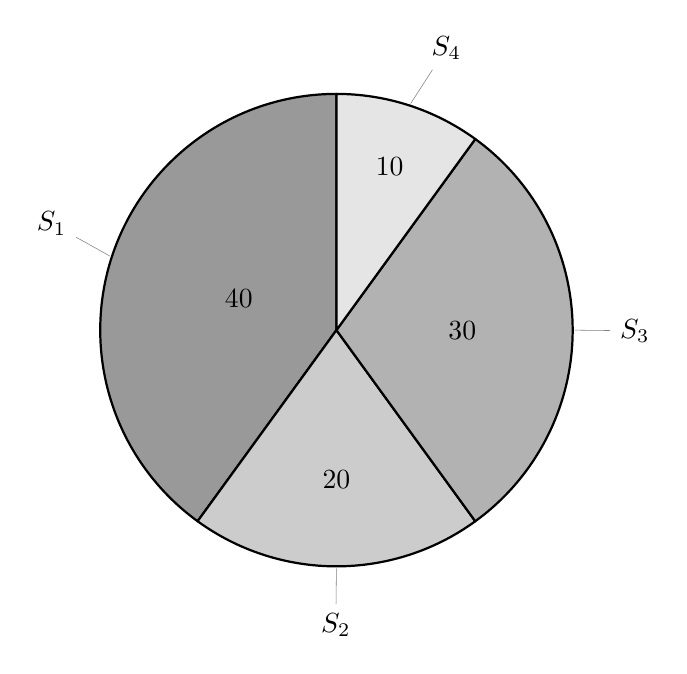
\begin{tikzpicture}
\pie [text=pin, rotate = 90, before number =, after number =,
      color={black!40,black!20,black!30,black!10}]
    {40/$S_{1}$, 20/$S_2$, 30/$S_3$, 10/$S_4$}
\end{tikzpicture}

}%

\bigskip

\resizebox{.3\textwidth}{!}{%
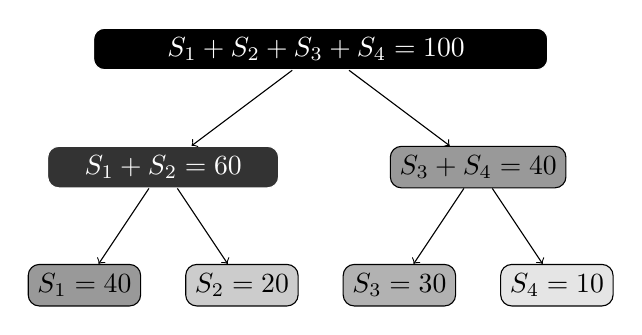
\begin{tikzpicture}[sibling distance=4cm,
  every node/.style = { shape=rectangle, rounded corners,
    draw, align=center, top color=white, bottom color=blue!20}]

\node[color=white, top color=black!100, bottom color=black!100]
     {\ \ \ \ \ \ \ \( S_1 + S_2 + S_3 + S_4 = 100 \) \ \ \ \ \ \ \ }
     child[->]
          { node[color=white, top color=black!80, bottom color=black!80]
                {\ \ \ \( S_1 + S_2 = 60 \)\ \ \ }
                child[sibling distance=2cm]
                     { node[top color=black!40, bottom color=black!40] {\( S_1 = 40 \)}}
                child[sibling distance=2cm]
                     { node[top color=black!20, bottom color=black!20] {\( S_2 = 20 \)}}
          }
     child[->]
          { node[top color=black!40, bottom color=black!40]
                {\(S_3 + S_4 = 40 \)}
                child[sibling distance=2cm]
                     { node[top color=black!30, bottom color=black!30] {\( S_3 = 30 \)}}
                child[sibling distance=2cm]
                     { node[top color=black!10, bottom color=black!10] {\( S_4 = 10 \)}}
          };
\end{tikzpicture}
}%

\caption{Imagining a spin dial as a tree. Segments
are sized in proportion to escrow stakes.}
  \label{fig:spinner}
\end{figure}


%\begin{figure}[h!]
%\centering
%
%\begin{tikzpicture}
%\pie [text=pin, rotate = 90, before number =, after number =,]
%    {40/Stake 1, 20/Stake 2, 30/Stake 3, 10/Stake 4}
%\end{tikzpicture}
%
%\bigskip
%
%\begin{tikzpicture}[sibling distance=4cm,
%  every node/.style = { shape=rectangle, rounded corners,
%    draw, align=center, top color=white, bottom color=blue!20}]
%
%\node{\ \ 100 (40 + 30 + 20 + 10)\ \ }[->]
%  child[->]{ node {\ \ \ 60 (40 + 20)\ \ \ }
%    child[sibling distance=2cm]{ node[bottom color=blue] {40}}
%    child[sibling distance=2cm]{ node[bottom color=cyan] {20}}
%  }
%  child[->]{ node {40 (30 + 10)}
%    child[sibling distance=2cm]{ node[bottom color=yellow] {30}}
%    child[sibling distance=2cm]{ node[bottom color=orange] {10}}
%  };
%\end{tikzpicture}
%
%\caption{Imagining a spin dial as a tree. Segments
%are sized in proportion to escrow stakes.}
%  \label{fig:spinner}
%\end{figure}


In practice a binary tree of participants is formed, in some consistent order, where each interior node represents the sum of all its sub-node stakes. The topmost node of the tree shows the full sum of all stakes represented in the tree, with all participants located in leafs. Branching decisions begin at the top node of the tree and descend toward leafs using the random value as a probe of the interval described by the partial sum at each node, with the division between left and right based on the relative weights of its two subtrees. Descent continues until meeting a leaf node, and declaring that node the winner of the election. 

If the random probe value is converted into a fractional value of its range, and each interior node is relabeled with its division fractional value, then it is simple to choose left or right subnodes based on a single comparison between the two fractional values.

That this works can be seen by noting that every interior node of the tree serves both as denominator to nodes below, and as numerator to connections above, hence cancelling out. The final probability for any participant winning becomes the same as their escrow stake divided by the sum of all participant escrow stakes.

\subsubsection{Self-Healing Protocol}
Once elected, the new leader forms the necessary Cosi trees and Randherd groups, and begins assembling a new block for the duration of the epoch until the next election round. There is implicit consensus on the election result as Cosi requests become satisfied using newly formed groups.

We try to construct a protocol that is self-healing in the event that failures arise. In normal circumstances, elections are held on a schedule, and all stakeholders recognize the signal to hold a new election. 

There must be a balancing of the period between elections and the length of time it takes to assemble and validate blocks. The larger the block, in number of transactions to be verified, the longer it will take. Beyond some size, that administrative duration would exceed the interval between Randherd beacon outputs.

Each stakeholder knows all the other participants in the escrow system, and can run the election for themselves upon seeing the random value of the election signal. Election signals arrive by way of authenticated randomness, and all stakeholders should know which other participants can sign the randomness. Outsider trolls will be ignored.

All nodes should be able to agree on election outcome, but if not, then one of two things could happen. First, if a stakeholder thinks it won the election but was mistaken, then any attempts at forming new Cosi networks by the faux leader would be silently rejected by others, and it would fail to obtain a consensus on any new requests. If that happens, the rejected leader should resynchronize its list of participants, rerun its own election, and join back in after agreeing on the outcome. 

Second, a stakeholder might think that someone else had won the election. In that case, it would silently reject Cosi formation requests by whomever had actually won, and never see any requests from whom it thought it should. If this happens for two consecutive election cycles, then something may be amiss, and it should attempt to re-synchronize its list of participants.

If a stakeholder wins an election but is absent or comes under attack, it may not respond to its own election as leader, or block assembly activities will cease in that epoch. Any Cosi witness can call for a new early election, and after $(2 f+1)$ such calls have been seen, each from different nodes, a new election cycle ensues. (Byzantine attacks may try this as well, hence the threshold.)

Honest stakeholder nodes will typically register a complaint after seeing no activity for longer than an adaptive threshold based on recent past rates. An exponential average could be used for this purpose. Early elections will use the last random election probe against a decision tree that excludes the previously elected leader.

\subsubsection{Digression on Network Protocols}
Our network protocol dictates that all messages must be authenticated with sender's signature or else the message will be ignored on delivery. Higher level portions of the system are completely network agnostic with regard to method of transport. It does not matter to Cosi, for example, whether messages arrive by UDP, Gossip, HTTP, or any other method.

But however messages arrive, the port interface takes care to validate incoming message signatures, and if they fail, the messages are ignored. 

Signatures are merely a first line of defense against network trolls. But they do nothing other than to vouch for the sender as having a legitimate key pair. They cannot certify proper contents, nor censor illegitimate messages. 

Getting past signature validation simply means that the structure of the message packet was such that a signature portion could be identified, along with a public key, and together with the hash of the message body, everything seems to check as a non-forgery from the claimed sender.

Some protocols might choose to discard the incoming signature portion after verification. Others might optimize forwarding by retaining the original packet for forwarding, rather than rewrapping its message body with a new signature. 

So it is quite possible that a message originating from one public key will arrive at its destination with the signature of an intermediary.

With Gossip it is also possible that the same message will arrive more than once, by different routes. We must filter incoming messages to ignore repeats. Messages should carry the hash of their contents, or become hashed at delivery, as a timeless identifier for this purpose. But there will be a practical limit to the depth of this filtering. It should be deep enough to cover all but some miniscule portion of likely transport delays.

And since the hash of the message might bear little relationship to its original signature, we cannot rely solely on the signature for this filtering.

\subsubsection{Mostly-Stateless Design}
In the interest of overall system stability and simplicity, a mostly stateless architecture seems desirable. Communications are often by {\em{Gossip}} protocol, and so no hard time limit can easily be stated for communication delays.

So rather than defining node states with a transition diagram between states, we make each communicated message  carry information about its purpose along with relevant identifying information.  

Immediately after a leader election, each node should determine its role for the new epoch. 
\begin{itemize}
    \item If elected leader, then begin next block assembly. 
    \item If the node should become a member of a RandHerd group, then start running the protocol within its group.
    \item If the node should become a Cosi witness node, then start a timeout timer. If that timeout ever fires, then it is time to call for a new election. But incoming messages can restart or cancel the timeout timer.
    \item Otherwise, the node is on standby for the next election cycle. Nodes in standby can ignore almost all messages, but must pay attention to election related messages.
\end{itemize}  

All stakeholder nodes must pay attention to election messages:
\begin{itemize}
\item New Election Message - Run an election with the random value provided in the election message, and determine next role for this node - one of Leader, Cosi participant, RandHerd participant, or standby. Reset the counter of calls for new election.

\item Call For New Election Message - Increment the count, $n$,  of such calls seen from different nodes, and if $n \ge 2 f +1$, then run another election round based on the last election random value, with a decision tree sans current leader node. Determine new leader and next role for this node.  Reset the counter of calls for new  election.

Note that repeated calls from the same public key must be ignored. That extends beyond the hash filtering for duplicate incoming messages.  An attacker might otherwise flood the system with calls for new election that overcome the incoming message filtering. So, in fact, such messages must be signed by the public key holder.\footnote{All incoming message are already signed with the signature of the sender. But that signature might be discarded by the port manager, once validated. Nothing otherwise dictates what can be sent by any node.  And recall that the signature might have no relation to the public key in the message.

Furthermore, sender might be an attacker who is able to sign network messages, and who attempts to forge attribution to other public keys. 
We need to know that the public key of the complainant was legitimately used to call for new election.}
\end{itemize}

For nodes in a Cosi group there are five different events that have any relevance to each witness node: 
\begin{itemize}
\item Consensus Prepare Message - Attempt to validate the message. If valid, affix signature and send back to leader. Validation includes checking that the message arrived from the current leader node. If not, then just ignore the message. If the message was valid, then restart the timeout timer if it was running.

\item Consensus Commit Message - Check that the message arrived from the current leader. If so, affix a signature, send back to leader, and record the message in persistent store.

If the message arrived from someone, not the current leader, then it either already had enough signatures to become committed, and so it is now in the current blockchain. Or else, it failed to gain commit consensus and it was dropped. Either way, we can just ignore it.

Leave the timeout timer running.

\item Self Timeout - Gossip a call for new elections. Do not restart timeout timer. Message gossipped must include the public key of this node for accounting purposes.

\item New Election Message - Kill the timeout timer, then proceed as usual for a new election message.

\item Call For New Election Message - Increment the count, $n$,  of such calls seen from different nodes, and if $n \ge 2 f +1$, then kill the timeout timer, and proceed as usual for early elections.
\end{itemize}

Nodes in a RandHerd group must pay attention to the following messages:
\begin{itemize}
\item TBD...
\end{itemize}

%%%%%%%%%%%%%%%%%%%%%%%%%%%%%%%%%%%%%%%%%%%%%%%%%%%
\subsection{Cryptographic Sortition}
Sortition\cite{algorand} is the process of randomly selecting members for Cosi networks and Randherd groups, based on stake weighting. We described one type of sortition event in the description of blockchain leader election. The process is repeated for selection of other duties. Random values for sortition probing are developed using VRF's to prove fairness in making selections.

As the outcome of selections becomes known, those stakeholders must be removed from the selection tree before holding additional rounds. The purpose of sortition rounds specifies roles, each of which may have different threshold requirements in number of selected participants. Roles specify the purpose of selection, such as for Cosi networks, Randherd groups, and so forth.

%%%%%%%%%%%%%%%%%%%%%%%%%%%%%%%%%%%%%%%%%%%%%%%%%%%

\subsection{Safe Hierarchical Keying}

In current blockchain designs which utilize simple Elliptic Curve cryptography, the possibility of producing subkeys from a master public key is presented. But that is wholly unsafe in the event that a decryption key is also generated for a derived public key. A simple bit of finite field arithmetic is all it takes to discover the original master private key.

With PBC we can safely generate both public and private keys without exposing our master private key. This is also known as Identity-Based Encryption (IBE). But unlike conventional presentations of IBE, we do not rely on a trusted third party for the generation of our keying. Rather, we view the master key holder as the only entity that should be entitled to generate new decryption keys. 

Anyone can generate new public keys at any time, based on previously known public keys.
But in order to obtain a decryption key for the new public keys, you must ask the primary secret key holder for a decryption key. Doing so puts the primary key holder at no risk for exposing his or her private key.

A new public key can be generated by asking for a subkey of a given public key, using an arbitrary identity value to identify that subkey. The new public key is computed as 
$$ P_{id} = Z_r(H(id)) \, V + P$$ 
for identity $id$, generator $V \in G_2$, public key $P \in G_2$, and where $Z_r(H(id)) \in Z_r$ is the element of the field that corresponds to the hash of the supplied identity. 

You can use this public key to encrypt a message by making use of the hash of a pairing value as an XOR mask against a message $$E(msg) = msg \oplus H(g^x)$$ where $x = Z_r(H(msg, id)) \in Z_r$, and pairing element 
$$g^x = e(U, x \, V)$$
for generator $U \in G_1$, generator $V \in G_2$. The message is transmitted as the triple $(E(msg), X, id)$, with $X = x \, P_{id} \in G_2$.

In order to produce a decryption key for that new public key, the primary key holder computes $$S_{id} = \frac{1}{s + Z_r(H(id))} \, U \in G_1$$ for secret key $s \in Z_r$. Producing a decryption key in $G_1$ ensures, by difficulty of ECDLP, that our master private key remains safe against exposure.

Homomorphism allows us to see that the pairings 
$$
\begin{align}
    e(S_{id}, X) &= e(\frac{1}{s + Z_r(H(id))}\, U, x\,(Z_r(H(id)) \, V + P)) \\
    &= e(U, x\, V) = g^x
\end{align}$$ 
which allows us to recreate the XOR mask and decrypt to the original message 
$$msg = E(msg) \oplus H(g^x)$$ 

Verification of the message is done by computing $x = Z_r(H(msg, id))$ and checking that 
$$x\, (Z_r(H(id))\, V + P) = X \in G_2$$

In this form, a new private key cannot be used to sign messages in the usual manner as for BLS signatures with the master private key, because we have $P_{id} \neq s_{id} \, V$. But it does furnish a way to encrypt and decrypt messages by using the hash of the pairing result. This technique has been dubbed SAKKE by its authors Sakai-Kasahara\cite{sakke}. We have extended SAKKE encryption to indefinite length by using successive SHA3 hashes on the pairing field result and an increasing index value.
%%%%%%%%%%%%%%%%%%%%%%%%%%%%%%%%%%%%%%%%%%%%%%

% ensure same length columns on last page (might need two sub-sequent latex runs)
\balance

% The following two commands are all you need in the
% initial runs of your .tex file to
% produce the bibliography for the citations in your paper.
\bibliographystyle{abbrv}
% \bibliography{yellowpaper}  

\begin{thebibliography}{99}

\bibitem{bn}Paulo S. L. M. Barreto and Michael Naehrig
{\em{Pairing-Friendly Elliptic Curves of Prime Order}}

\bibitem{bulletproofs} Benedikt Bunz, Jonathan Bootle, Dan Boneh, Andrew Poelstra, Pieter Wuille, and Greg Maxwell
{\em{Bulletproofs: Short Proofs for Confidential Transactions and More}}

\bibitem{scrape}Ignacio Casudo and Bernardo David, 
{\em{ SCRAPE: Scalable Randomness Attested by Public Entities}} 

\bibitem{vrf}Yevgeniy Dodis and Aleksandr Yampolskiy, 
{\em{A Verifiable Random Function With Short Proofs and Keys}}

\bibitem{algorand}Yossi Gilad, Rotem Hemo, Silio Micali, Georgios Vlachos, Nickolai Zeldovich,
{\em{Algorand: Scaling Byzantine Agreements for Cryptocurrencies}}

\bibitem{thesis} Ben Lynn, PhD Thesis, 
{\em{On the Implementation of Pairing-Based Cryptosystems}}, June 2007

\bibitem{lib} Ben Lynn, PBC Library, 
https://crypto.stanford.edu/pbc/download.html

\bibitem{bls} Ben Lynn, 
{\em{BLS Signatures}}, 
https://crypto.stanford.edu/pbc/manual/ch02s01.html

\bibitem{vrf2}Silvio Micali, Michael Rabin, Salil Vadhan, 
{\em{Verifiable Random Functions}}

\bibitem{sakke}Sakai-Kasahara, 
{\em{IETF RFC 6508 Sakai-Kasahara Key Encryption (SAKKE)}} 

\bibitem{cosi}Ewa Syta, Iulia Tamas, Dylan Visher, David Isaac Wolinsky, Philipp Jovanovic, Linus Gasser, Nicolas Gailly, Ismail Khoffi, Bryan Ford, 
{\em{Keeping Authorities ``Honest or Bust'' with Decentralized Witness Cosigning}}

\bibitem{randhound} Ewa Syta, Philipp Jovanovic, Eleftherios Kokoris Kogias, Nocals Gailly, Linus Gasser, Ismail Khoffi, Michael J. Fisher, Bryan Ford, 
{\em{Scalable Bias-Resistant Distributed Randomness}}

\bibitem{tpm} Youlian Tian, Changgen Peng, Jianfeng Ma, 
{\em{Publicly Verifiable Secret Sharing Scheme Using Bilinear Pairings}}

\end{thebibliography} 
\end{document}
